\documentclass[a4paper,11pt]{article}
\usepackage[T1]{fontenc}
\usepackage[utf8]{inputenc}
\usepackage{lmodern}
\usepackage{polski}
\usepackage{tikz}
\usepackage{pgf}
\usepackage{siunitx,booktabs}
\sisetup{
    table-auto-round
}

\title{Sprawozdanie}
\author{Bartosz Zasieczny}

\begin{document}

\maketitle
\tableofcontents

\section{Zadanie}
Korzystając z omówionych na wykładzie iteracyjnych metod aproksymacji pierwiasków, zaproponować sposób wyznaczania \textbf{\emph{ekstremum lokalnego}} funkcji \( f \in C^1[a,b] \). Wykonać eksperymenty m. in. dla:
\begin{enumerate}
  \setcounter{enumi}{-1}
  \item \( f(x) = sin(2 \pi x) \), \( x \in [0,1] \); 
  \item \( f(x) = e^{-x^2} \), \( x \in [-1, 1] \); 
  \item\( f(x) = \frac {x} {1+x^2} \), \( x \in [0,10] \); 
  \item\( f(x) = x^2 + x - 1 \), \( x \in [-1,2] \).
\end{enumerate}

\section{Aparat matematyczny}
  W poszukiwaniu ekstremów funkcji będziemy używać poniższych metod. Niektóre z nich pozwalają na znalezienie ekstremum wprost, inne będą skupiać się na poszukiwaniu miejsca zerowego pierwszej pochodnej funkcji tam gdzie to możliwe.
  \subsection{Metoda Newtona}
  \textbf{Metoda Newtona} polega na iteracyjnym wyznaczaniu kolejnych przybliżeń pierwiastka \( f(x) \) poprzez: 
  \begin{itemize}
    \item znalezienie stycznej do jej wykresu w punkcie \(x_i\) (zaczynając od punktu startowego \(x_0\)); 
    \item biorąc wartosć dziedziny w punkcie przecięcia stycznej z osią \(X\) za \(i+1\)-sze przyblizenie pierwiastka (czyli \( x_{i+1} \)).
  \end{itemize}
  Kroki powtarzamy aż do otrzymania wymaganej precyzji.
  Kolejne przybliżenia \( x_{i+1} \) wyznaczamy za pomocą wzoru:
  $$ x_{i+1} = x_i - \frac {f(x_i)} {f'(x_i)} $$
  \subsubsection{Uwagi}
  
  \begin{itemize}
    \item Charakterystyka tego zadania uniemożliwia użycie samej metody Newtona - dla pewnych danych może ona wskazać przybliżenia pierwiastka \( f(x) \) spoza pożądanego przedziału. Problemem też jest dobór odpowiedniego punktu startowego - dlatego w przypadku tego zadania należy stosować tę metodę tylko po wstępnym przybliżania pierwiastka funkcji przez inne metody iteracyjne.
    \item W przypadku tego zadania każda badana funkcja musi posiadać co najmniej dwie pochodne.
  \end{itemize}
  
  \subsection{Metoda bisekcji}
  Dla funkcji \( f(x) \) ciągłej w przedziale \( [a,b] \) i przyjmującej na jego końcach wartości o różnych znakach (\( f(a) f(b) < 0 \)) należy wykonać następujące kroki:
  \begin{enumerate}
    \item sprawdzić, czy srodek przedziału jest pierwiastkiem funkcji (sprawdzić czy \( f(x) \) dla wartości dziedziny \(x_0 = \frac {a + b} {2} \) ma wartość \(f(x_0) = 0 \);
    \item jeśli tak, to zakończyć algorytm i zwrócić \(x_0\);
    \item w p. p. sprawdzić który z przedziałów (\( [a, x_0] \) czy \( [x_0, b] \)) spełnia własnosć \( f(a')f(b') < 0 \) i zastosować do niego pierwszy krok algorytmu.
  \end{enumerate}
  
  \subsection{\emph{Regula falsi}}
  Metoda \emph{fałszywej prostej} wyznacza przyblizenia pierwiastka \( f(x) \) spełniającej następujące założenia w przedziale \([a, b]\):
  \begin{itemize}
    \item \( f(x) \) jest ciągła w przedziale \( [a,b] \);
    \item \( f(x) \) w przedziale \( [a,b] \) ma \textbf{dokładnie jeden} pierwiastek;
    \item \( f(x) \) na końcach przedziału \( [a,b] \) przyjmuje różne znaki wartości \\(\( f(a) f(b) < 0 \));
    \item \( \forall_{x \in [a.b]} \: \exists_{f'(x)} \wedge \exists_{f''(x)}\);
    \item \( \forall_{x', x''\in [a,b]}\; sgn\: f'(x') = sgn \: f'(x'') \: \wedge \: sgn \: f''(x') = sgn \: f''(x'') \).
  \end{itemize}
  Aby wyznaczyć przybliżenie pierwiastka nalezy wykonać nastepujące kroki:
  \begin{enumerate}
    \item przez punkty \(A = (a, f(a))\) i \(B = (b, f(b))\) przeprowadzana jest prosta;
    \item punkt przecięcia \(x_i\) osi \(X\) jest przyblizeniem pierwiastka;
    \item jeśli precyzja przybliżenia jest zadowalająca to kończymy algorytm;
    \item w p. p. wybierany jeden z przedziałów (\( [a, x_i] \) czy \( [x_i, b] \)) taki, który spełnia własnosć \( f(a')f(b') < 0 \) i stosujemy do niego pierwszy krok algorytmu.
  \end{enumerate}
  \subsubsection{Wzory}
    $$ x_{0}=\frac{af(b)-bf(a)}{f(b)-f(a)} $$
    $$ x_{i+1}= \left \{ \begin{array}{lll} 
    \displaystyle{\frac {x_i f(a) - a f(x_i)} {f(a) - f(x_i)}} & \textrm{gdy} & f(a)f(x_i) \le 0 \\ \\
    \displaystyle{\frac {x_i f(b) - b f(x_i)} {f(b) - f(x_i)}} & \textrm{gdy} & f(b)f(x_i) < 0 
  \end{array}\right. $$
  dla \( i = 1,2,... \)
  
  \subsection{Metoda \emph{złotego podziału}}
    Ta metoda w odróżnieniu od poprzednich pozwala szukać lokalnego ektremum wprost, bez konieczności odwoływania się do pochodnych danej funkcji i poszukwiania ich zer. Żeby funkcja \( f(x) \) mogła zostać zbadana za pomocą tej metody, musi być ona w przedziale \( [a,b] \), w którym poszukujemy ekstremum, \textbf{\emph{unimodalna}} -- tzn. ciągła i posiadać w tym przedziale dokładnie jedno ekstremum.
    \subsubsection{Algorytm}
    Pierwszy krok algorytmu:
    $$ \left\{\begin{array}{l}
    x_L^{(0)} := b^{(0)} - (b^{(0)}-a^{(0)})k \\ \\
    x_R^{(0)} := a^{(0)} + (b^{(0)}-a^{(0)})k
    \end{array}\right. $$
    
    Następnie iterujemy po przypadkach, aż do uzyskania zadowalającej precyzji:
    \begin{itemize}
      \item \( f(x_L^{(i)}) > f(x_R^{(i)}) \Rightarrow \left\{\begin{array}{l}
        a^{(i+1)} := x_L^{(i)} \\
        b^{(i+1)} := b^{(i)} \\
        x_L^{(i+1)} := x_R^{(i)} \\
        x_R^{(i+1)} := a^{(i+1)} + (b^{(i+1)}-a^{(i+1)})k
        \end{array}\right. \)
      \item \( f(x_L^{(i)}) < f(x_R^{(i)}) \Rightarrow \left\{\begin{array}{l}
        a^{(i+1)} := a^{(i)} \\
        b^{(i+1)} := x_R^{(i)} \\
        x_L^{(i+1)} := b^{(i+1)} - (b^{(i+1)}-a^{(i+1)})k \\
        x_R^{(i+1)} := x_L^{(i)}
        \end{array}\right. \)
    \end{itemize}
    Po zakończeniu iteracji, środek przedziału $[a,b]$ jest brany jako przybliżenie lokalnego ekstremum funkcji.
  \section{Badanie funkcji}
    Do wykonywania obliczeń używana jest arytmetyka w standardzie IEEE 754 \emph{double}.
    \subsection{Funkcja 0}
      Wzory i wykresy funkcji i pochodnych w podanym przedziale: \\ 
      \begin{center}
      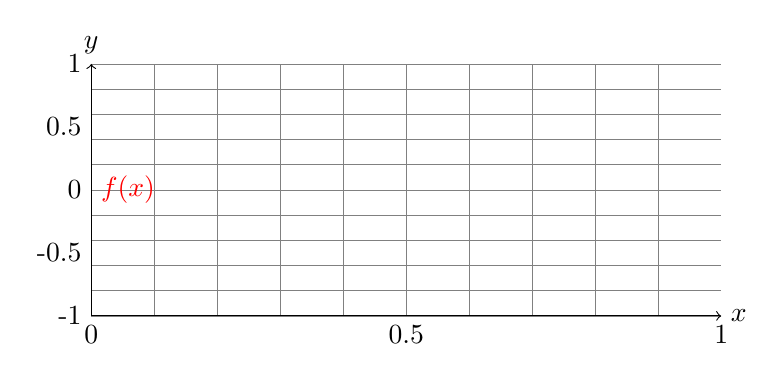
\begin{tikzpicture}[x=8cm,y=1.6cm]

        \def\xmin{0}
        \def\xmax{1}
        \def\ymin{-1}
        \def\ymax{1}

        \draw[style=help lines, ystep=0.2, xstep=0.1] (\xmin,\ymin) grid
        (\xmax,\ymax);

        \draw[->] (\xmin,\ymin) -- (\xmax,\ymin) node[right] {$x$};
        \draw[->] (\xmin,\ymin) -- (\xmin,\ymax) node[above] {$y$};

        \foreach \x in {0, 0.5 ,..., 1}
          \node at (\x, \ymin) [below] {\x};
        \foreach \y in {-1,-0.5 ,...,1}
          \node at (\xmin,\y) [left] {\y};

         \draw[color=red, domain=\xmin:\xmax] plot[id=f]
          function{sin(2*pi*x)} node [right] {$f(x)$};
  
      \end{tikzpicture}
      \end{center}
      $$ f(x) = sin(2 \pi x)  \textrm{,} \; x \in [0,1] $$
      \begin{center}
      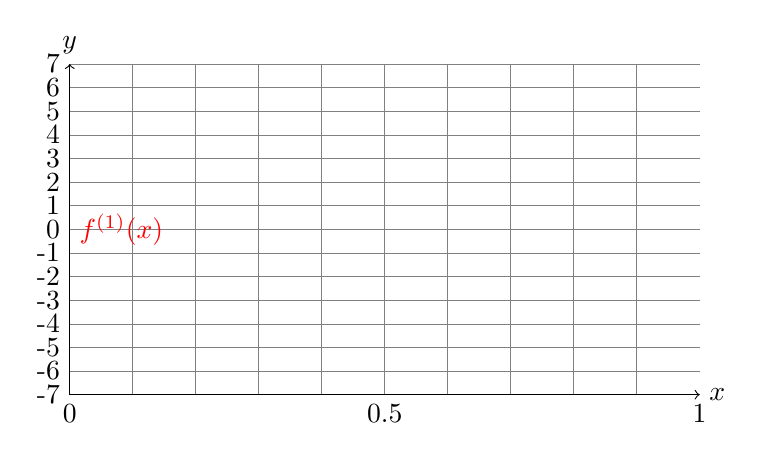
\begin{tikzpicture}[x=8cm,y=0.3cm]

        \def\xmin{0}
        \def\xmax{1}
        \def\ymin{-7}
        \def\ymax{7}

        \draw[style=help lines, ystep=1, xstep=0.1] (\xmin,\ymin) grid
        (\xmax,\ymax);

        \draw[->] (\xmin,\ymin) -- (\xmax,\ymin) node[right] {$x$};
        \draw[->] (\xmin,\ymin) -- (\xmin,\ymax) node[above] {$y$};

        \foreach \x in {0, 0.5 ,..., 1}
          \node at (\x, \ymin) [below] {\x};
        \foreach \y in {-7,-6 ,...,7}
          \node at (\xmin,\y) [left] {\y};

         \draw[color=red, domain=\xmin:\xmax] plot[id=fd]
          function{2 * pi * cos(2*pi*x)} node [right] {$f^{(1)}(x)$};
  
      \end{tikzpicture} 
      \end{center}
      $$ f^{(1)}(x) = 2 \pi \cdot cos(2 \pi x) $$
      \begin{center}
      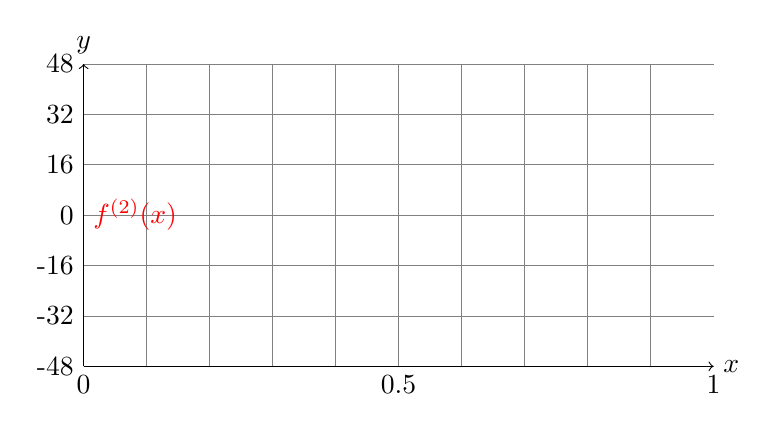
\begin{tikzpicture}[x=8cm,y=0.04cm]

        \def\xmin{0}
        \def\xmax{1}
        \def\ymin{-48}
        \def\ymax{48}

        \draw[style=help lines, ystep=16, xstep=0.1] (\xmin,\ymin) grid
        (\xmax,\ymax);

        \draw[->] (\xmin,\ymin) -- (\xmax,\ymin) node[right] {$x$};
        \draw[->] (\xmin,\ymin) -- (\xmin,\ymax) node[above] {$y$};

        \foreach \x in {0, 0.5 ,..., 1}
          \node at (\x, \ymin) [below] {\x};
        \foreach \y in {-48,-32 ,...,48}
          \node at (\xmin,\y) [left] {\y};

         \draw[color=red, domain=\xmin:\xmax] plot[id=fd2]
          function{-4 * pi**2 * sin(2*pi*x)} node [right] {$f^{(2)}(x)$};
  
      \end{tikzpicture} 
      \end{center}
      $$ f^{(2)}(x) = -4 \pi^2 \cdot sin(2 \pi x) $$
      \begin{center}
      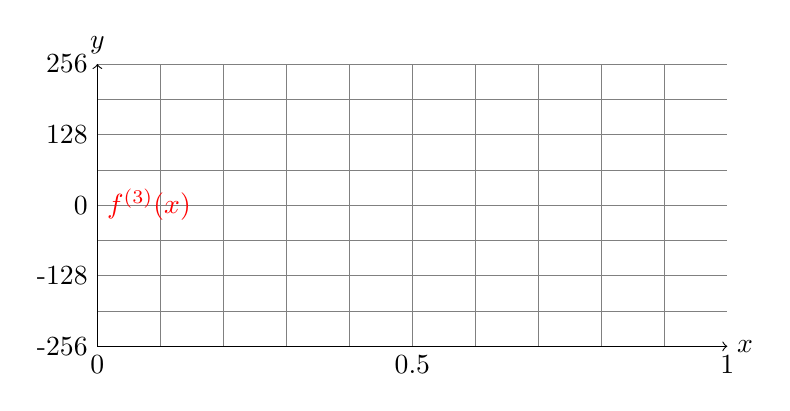
\begin{tikzpicture}[x=8cm,y=0.007cm]

        \def\xmin{0}
        \def\xmax{1}
        \def\ymin{-256}
        \def\ymax{256}

        \draw[style=help lines, ystep=64, xstep=0.1] (\xmin,\ymin) grid
        (\xmax,\ymax);

        \draw[->] (\xmin,\ymin) -- (\xmax,\ymin) node[right] {$x$};
        \draw[->] (\xmin,\ymin) -- (\xmin,\ymax) node[above] {$y$};

        \foreach \x in {0, 0.5 ,..., 1}
          \node at (\x, \ymin) [below] {\x};
        \foreach \y in {-256,-128 ,...,256}
          \node at (\xmin,\y) [left] {\y};

         \draw[color=red, domain=\xmin:\xmax] plot[id=fd3]
          function{-8 * pi**3 * cos(2*pi*x)} node [right] {$f^{(3)}(x)$};
  
      \end{tikzpicture} 
      \end{center}
      $$ f^{(3)}(x) = -8 \pi^3 \cdot cos(2 \pi x) $$
      
      Z wykresów można wywnioskować, że w tym przedziale funkcja $ f \in C^3 $. Na wykresie $ f $ można zauważyć, że w przedziale $[0,1]$ ma ona 2 ekstrema -- jedno minimum, jedno maksimum. Sugeruje to możliwość użycia metody \emph{złotego podziału}. Niestety $f^{(2)}$ i $f^{(3)}$ nie mają takich samych znaków dla każdej wartości argumentu z zadanego przedziału -- użycie metody \emph{regula falsi} będzie zatem bardzo utrudnione, zatem ją pominiemy dla tej funkcji. Możemy natomiast użyć metody bisekcji, ew. łącząc ją z metodą Newtona (trzeba jednak uważać, gdyż na końcach przedziału $f^{(2)}(0) = 0$ i $f^{(2)}(1) = 0$ -- nie mozemy użyć $ x = 0 $ i $ x = 1 $ jako punktów startowych tej metody).
      
      \subsubsection{Metoda \emph{złotego podziału}}
      Polecenie: \texttt{./main -m golden\_section -f 0 -s 0 1 -i 50 -error 10e-8} \\
      \begin{center}
      \begin{tabular}{S[table-format=1.0]S[table-format=-1.9]S[table-format=-1.15,table-auto-round=false]}
        \toprule
        {$i$}                & {$x_i$}               & {$f(x_i)$}            \\ \midrule
          0 & 0.69098300562505254874 & -0.93203242381322759513 \\
          1 & 0.80901699437494745126 & -0.93203242381322770616 \\
          2 & 0.73606797749978958301 & -0.99617104086482766157 \\
          3 & 0.78115294937452672830 & -0.98090406160281717884 \\
          4 & 0.75328890437410611636 & -0.99978649070871195015 \\
          5 & 0.73606797749978958301 & -0.99617104086482766157 \\
          31 & 0.75000003172107387872 & -0.99999999999998012701 \\
          32 & 0.74999999251167026593 & -0.99999999999999888978 \\
          33 & 0.75000001674441429955 & -0.99999999999999444888 \\ \bottomrule
        \end{tabular}
    \end{center}
    
    Metoda \emph{złotego podziału} dla tej funkcji osiąga wymaganą precyzję (badany przedział jest mniejszy niż $10^{-8}$) dopiero po 34 iteracjach. W ten sposób znaleźliśmy przyblizenie tylko lokalnego minimum funkcji $ f(x) = -1\textrm{,}\; x = 0.75 $ i błąd przyblizenia wynosi $ |x_{33} - x| \approx 0.00000001674441429955 $. \\
    Chcąc przybliżyć minimum nalezy wykonać to samo polecenie dodając paramatr \texttt{-e max}. Lokalne maksimum funkcji znajduje się w $ x = 0.25 $ i $ f(x) = 1 $ - aby otrzymać wynik o takiej samej precyzji należy wykonać dokładnie tyle samo iteracji i błąd przybliżenia jest bardzo zbliżony. Trzeba jednak pamiętać, że dokładność przyblizeń w przypadku tej funkcji zależy nie tylko od precyzji arytmetyki, ale również od dokładności reprezentacji piczby $\pi = 3.14159265358979323846$ (reprezentacja w \texttt{cmath}). \\
    Dla tej funkcji metoda \emph{złotego podziału} daje wyniki o rządanej precyzji po dość dużej liczbie iteracji. Aby otrzymać precyzję rzędu $10^{-16}$ program musi wykonać 72 iteracje.
    \subsubsection{Użycie metody \emph{złotego podziału} jako wstęp do metody Newtona}
    Warto tej metody użyć jako wstęp do metody Newtona. Weźmy 6-tą iterację z powyższej tabeli ($ i = 5 $) i użyjmy jej jako punkt startowy do metody Newtona (polecenie: \texttt{./main -m newton -f 1 -d 2 -x 0.75328890437410611636 -error 10e-8}). Otrzymujemy następujące dane:
     \begin{center}
      \begin{tabular}{S[table-format=1.0]S[table-format=-1.9]S[table-format=-1.15,table-auto-round=false]}
        \toprule
        {$i$}                & {$x_i$}               & {$f(x_i)$}            \\ \midrule
         0 & 0.75328890437410611636 & 0.12983149947540237323 \\
         1 & 0.74999953176226419327 & -0.00001848528487583362 \\
         2 & 0.75000000000000011102 & 0.00000000000000442639 \\ \bottomrule
      \end{tabular}
    \end{center}
  Otrzymujemy w tym wypadku dość szybko (tylko 3 iteracje!) dane bardzo dokładne (błąd: $ |x_2 - x| \approx 0.00000000000000011102 $) przybliżenie, które jest znacznie lepsze od uzyskanego na drodze zasosowania samej metody \emph{złotego podziału}. 
    
  \subsubsection{Metoda bisekscji}
  Uzywając tej metody musimy podzielić przedział na dwa: $ [0, 0.5] $ i $ [0.5, 1]$. Łatwo zauważyć, że metoda bisekcji zakończy się wtedy już po pierwszej iteracji, gdyż już wtedy dokładnie w połówach przedziałów będziemy mieć zera $f^{(1)}$. Aby się o tym przekonać wystarczy wykonać następujące polecenia:
  \begin{itemize}
    \item \texttt{./main -m bisection -f 1 -s 0 0.5 } - dla przedziału $[0, 0.5]$,
    \item \texttt{./main -m bisection -f 1 -s 0.5 1 } - dla przedziału $[0.5, 1]$
  \end{itemize}
  Jak widać nie ma sensu łączenie tej metody z metodą Newtona, gdyż daje ona bardzo dokładne wyniki w czasie rpaktycznie stałym dla tej funkcji i tych dnaych wejściowych.
      
      
  \section{Kompilacja i obsługa programu}
    \subsection{Wymagania}
    Aby skompilować program należy spełnić następujące wymagania dotyczące oprogramowania:
    \begin{itemize}
      \item kompilator $ G\!+\!+ $ w wersji 4.7 lub późniejszej - kompilator musi obsługiwać standard $ C^{++}11 $,
      \item obecność narzędzia GNU Make
    \end{itemize}
    Powyższe wymagania powinny być automatycznie spełnione w każdej aktualnej dystrybucji GNU/Linux.
    
    \subsection{Kompilacja}
    Należy przejść do katalogu \texttt{prog} i wykonać polecenie \texttt{make} - kompilacja wykona się automatycznie. W pliku \texttt{Makefile} podane są polecenia, które należy wykonać aby skompilować program ręcznie.
    
    \subsection{Obsługa programu}
    Program uruchamiamy za pomoca pliku \texttt{main}, po jego nazwie podając ciąg bedący kombinacją ponizszych parametrów:
    \begin{itemize}
      \item \texttt{-f <nr\_funkcji>} -- za pomocą tego argumentu wybieramy jedną z dostępnych funkcji - liczba przyporzadkowana funkcji to jej liczba porządkowa z treści zadania \( \cdot 3 \), dodanie 1 to pierwsza pochodna, dodanie 2 to druga pochodna,
      \item \texttt{-d <nr\_funkcji>} -- podobnie jak powyżej, tyle, że podajemy liczbę pochodnej,
      \item \texttt{-m <metoda>} -- wybór jednej z metod:
        \begin{itemize}
          \item \texttt{newton} -- metoda newtona (obowiązkowe parametry wywołania to \texttt{-f -d -x})
          \item \texttt{regula\_falsi} -- \emph{regula falsi} (obowiązkowe parametry to \texttt{-f -s})
          \item \texttt{bisection} -- bisekcja (obowiązkowe parametry to \texttt{-f -s})
          \item \texttt{golden\_section} -- metoda \emph{złotego podziału} (obowiązkowe parametry to \texttt{-f -s})
          \item \texttt{plot} -- "wykres" funkcji (punkty) (obowiązkowe parametry to \texttt{-f -s -step})
        \end{itemize}
      \item \texttt{-p <n>} -- wypisz wyniki z precyzją $n$ cyfr po przecinku (domyślnie 20),
      \item \texttt{-s <a> <b>} -- określ badany przedział od $a$ do $b$,
      \item \texttt{-x <y>} -- $y$ jako punkt startowy,
      \item \texttt{-e (min|max)} -- określ czy szukać lokalnego mininum czy maximum w przedziale (działa tylko z \texttt{-m golden\_section}, domyślnie \texttt{min}),
      \item \texttt{-error <e>} -- określ tolerancję błędu (domyślnie $ 10^{-10} $),
      \item \texttt{-step <s>} -- wielkość kroku przy obliczaniu punktów wykresu (działa tylko z \texttt{-m plot}, domyślnie 0.1),
      \item \texttt{-i <i>} -- ilość iteracji (domyślnie 20),
      
    \end{itemize}
    
    Przykład: szukamy lokalnego minimum dla pierwszej funkcji z zadania, w podanym przedziale, za pomocą metody \emph{złotego podziału}, z tolerancją błędu na poziomie $10^{-12}$, maksymalnie 30 iteracjami i precyzją 25 liczb po przecinku.
    \begin{center}
      \texttt{./main -f 0 -s 0 1 -m golden\_section -e 10e-12 -i 30 -p 25}
    \end{center}    
\end{document}
